\section{Overview}

To study how an agent should handle IT incidents whose cause is uncertain, this research adopts a design-and-evaluate approach~\cite{hevner2004}. It builds an artefact, a rule-constrained reinforcement learning agent together with the simulated environment in which it acts, and evaluates it in controlled experiments. The work proceeds in eight phases, shown in Figure~\ref{fig:pipeline}: specifying the problem, eliciting scenarios with the Directorate, building and validating the environment, encoding the rules, implementing the baselines, training the agents, running the experiments, and analysing the results.

\begin{figure}[H]
\centering
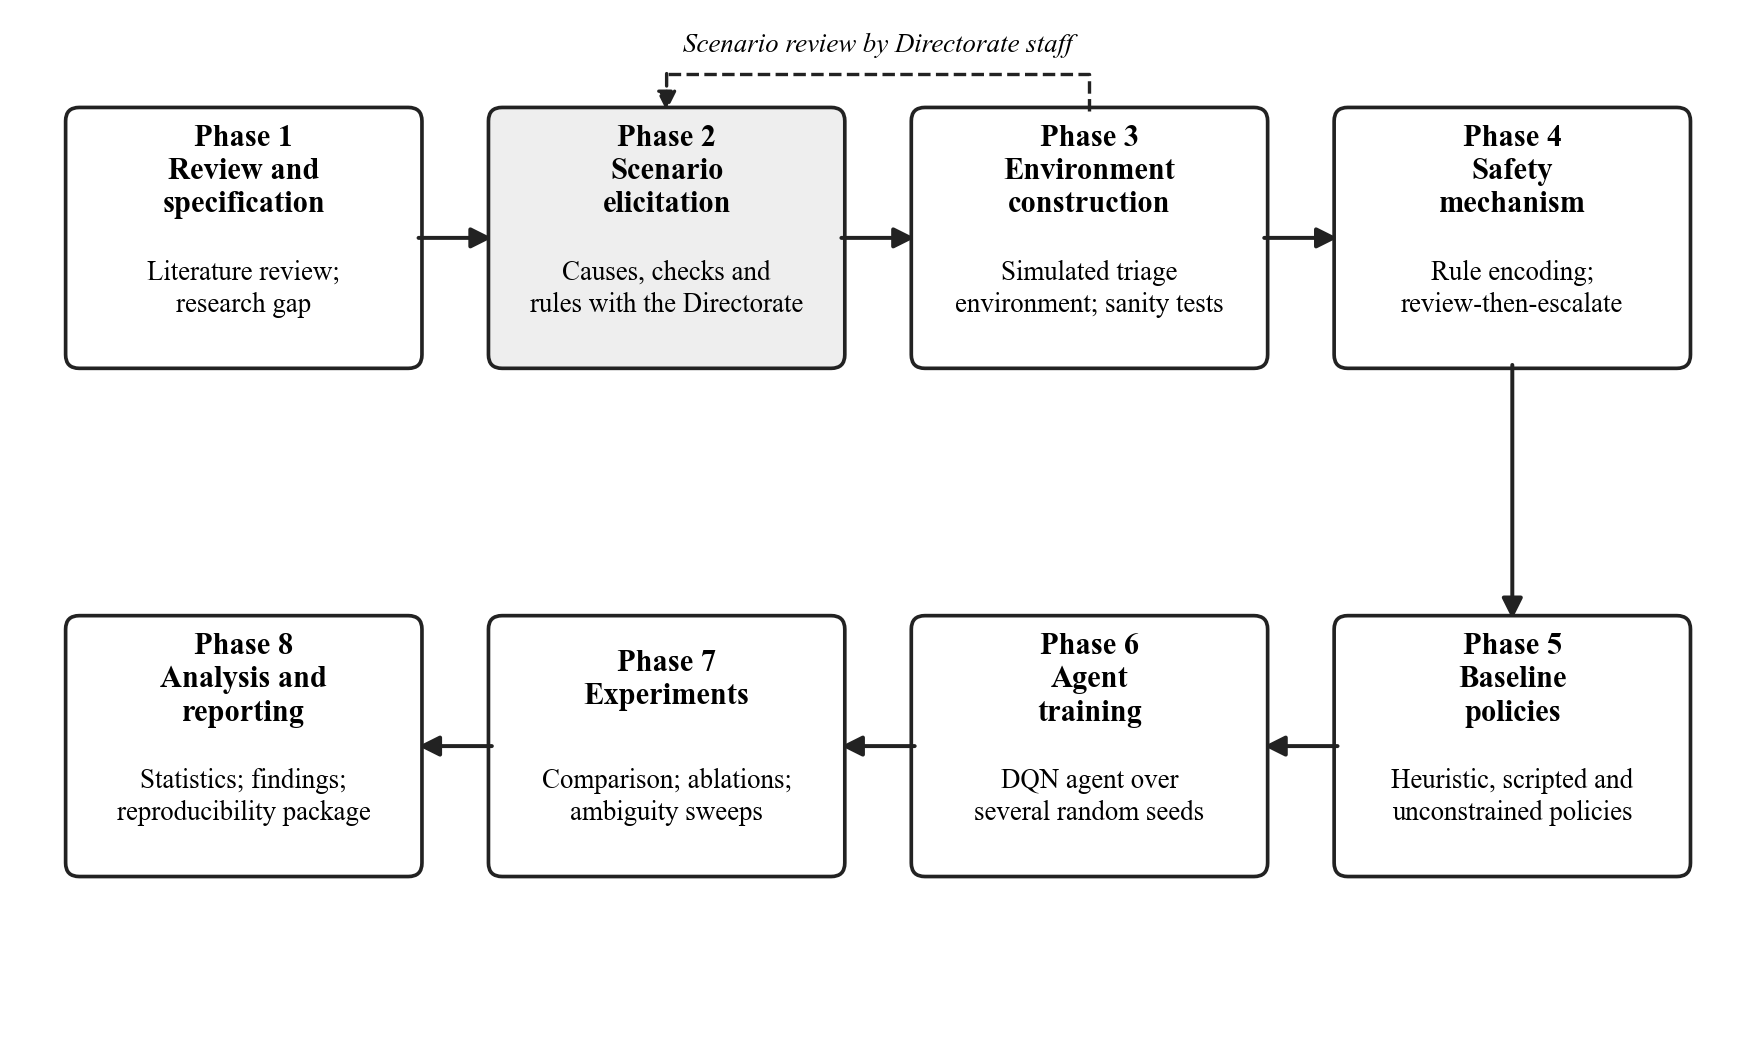
\includegraphics[width=\textwidth]{Figure_3_1_Research_Pipeline.png}
\caption{Research pipeline}
\label{fig:pipeline}
\end{figure}

The evaluation is conducted entirely in simulation, for two reasons. Realistic incident data is scarce and confidential~\cite{remil2024}, and simulation lets the level of ambiguity be set, held constant and varied, which live incidents would not allow. The agent is never connected to any system of the university. The framework will be implemented in Python, with the Gymnasium interface for the environment~\cite{towers2024} and the Stable-Baselines3 library for the learning algorithms~\cite{raffin2021}. No personal data, credentials or confidential details of the university's systems will enter the simulator, and staff participation will be voluntary and with consent.

\section{Data Collection}

The data for this research is a scenario model elicited from the Directorate of University ICT Services, not a dataset of incident records. The model will be elicited from Directorate staff using a structured workbook, and it will contain about 15 causes in four provisional categories (application and interface errors, authentication and access failures, database failures, and failures of infrastructure and external services), each with one correct fix; 20 diagnostic checks, such as an entry in the API logs, a value on the monitoring dashboard or the result of reproducing a failing request, each with an effort cost; a fixed list of about 10 symptoms, the signs reported when an incident is raised, such as a failed login or a slow page; and 10 operational rules.

Staff will give three sets of ratings on a five-point scale (never, rarely, sometimes, often, almost always) that is mapped to the probabilities 0.05, 0.25, 0.5, 0.75 and 0.95. For each pair of cause and check, they will rate how often the check is positive when that cause is present (300 ratings); for each pair of cause and symptom, how often the symptom is reported when that cause is present (150 ratings); and for each cause, how often it occurs, with the mapped values normalised to sum to one to give the prior over causes (15 ratings). Asking for verbal ratings keeps these 465 judgements manageable for practitioners. Any parameter that the elicitation does not supply will be set by the researcher and reported as such. After the environment is built, sample incidents will be shown to Directorate staff, who will judge whether they are plausible and whether the rules are stated correctly. The model will be revised and then frozen before any agent is trained, so that the scenarios cannot be adjusted in favour of the proposed agent.

\section{Problem Definition}
\label{sec:problem}

This section states the triage problem in general terms, independent of the numbers the Directorate will supply. Section~\ref{sec:environment} then gives the specific instance that is simulated.

\subsection{Triage as a Partially Observable Decision Problem:}

The triage of one incident is modelled as a finite-horizon partially observable Markov decision process (POMDP)~\cite{kaelbling1998},
\begin{equation}
\mathcal{M} = \langle \mathcal{S}, \mathcal{A}, \mathcal{T}, R, \Omega, \mathcal{O}, \gamma, H \rangle,
\end{equation}
whose elements are defined below.

\textbf{Causes, checks and context.} Let $\mathcal{C} = \{c_1, \dots, c_K\}$ be the set of possible causes of an incident, $\mathcal{D} = \{d_1, \dots, d_J\}$ the set of diagnostic checks, with check $d_j$ having cost $k_j > 0$, and $\mathcal{X}$ the set of incident contexts, such as whether the affected system is in production. The result of check $d_j$ is positive with a probability that depends on the cause:
\begin{equation}
\theta_{jm} = P(d_j = \text{positive} \mid c_m), \qquad j = 1, \dots, J, \quad m = 1, \dots, K.
\label{eq:likelihood}
\end{equation}
An incident also arrives with symptoms. Each of the $E$ symptoms is either present or absent, $\sigma_e \in \{0, 1\}$, and is reported with a probability that depends on the cause:
\begin{equation}
\varphi_{em} = P(\sigma_e = 1 \mid c_m), \qquad e = 1, \dots, E, \quad m = 1, \dots, K.
\label{eq:symptoms}
\end{equation}
The symptoms and the check results are assumed to be independent of one another given the cause.

\textbf{States ($\mathcal{S}$).} A state $s_t = (c, x, \boldsymbol{\sigma}, \mathbf{z}, \mathbf{q}_t)$ consists of the hidden cause $c \in \mathcal{C}$, the context $x \in \mathcal{X}$, the symptom vector $\boldsymbol{\sigma} \in \{0,1\}^E$, the vector $\mathbf{z}$ of check results, both drawn once at the start of the incident and unchanged afterwards, and the vector $\mathbf{q}_t \in \{0,1\}^J$ recording which checks have been requested by step $t$. The cause $c$ is never observed by the agent.

\textbf{Actions ($\mathcal{A}$).} The agent can request a check, recommend the fix for one cause, or escalate:
\begin{equation}
\mathcal{A} = \mathcal{A}_{\text{check}} \cup \mathcal{A}_{\text{fix}} \cup \{a_{\text{esc}}\}, \qquad
\mathcal{A}_{\text{check}} = \{a^{\text{chk}}_1, \dots, a^{\text{chk}}_J\}, \quad
\mathcal{A}_{\text{fix}} = \{a^{\text{fix}}_1, \dots, a^{\text{fix}}_K\},
\end{equation}
so that $|\mathcal{A}| = J + K + 1$.

\textbf{Transitions ($\mathcal{T}$).} The cause, context and check results are fixed for the whole episode. Requesting check $d_j$ sets $q_{t+1,j} = 1$ and reveals its result. Recommending a fix or escalating ends the episode, and so does reaching the step limit $H$, which is treated as an escalation.

\textbf{Observations ($\Omega$, $\mathcal{O}$).} At step $t$ the agent receives
\begin{equation}
o_t = (\mathbf{u}_t, \boldsymbol{\sigma}, x, t, \beta_t),
\end{equation}
where $u_{t,j} \in \{\text{not requested}, \text{unavailable}, \text{negative}, \text{positive}\}$ is the state of check $d_j$, $\boldsymbol{\sigma}$ is the vector of symptoms reported at the start, and $\beta_t \in \{0,1\}$ is set when the agent's previous proposal was blocked by the safety mechanism.

\textbf{Reward ($R$).} The reward expresses the costs that Chapter~1 attributed to each choice:
\begin{equation}
R(s_t, a_t) =
\begin{cases}
-k_j & \text{if } a_t = a^{\text{chk}}_j, \\
+r_{\text{correct}} & \text{if } a_t = a^{\text{fix}}_m \text{ and } c_m = c, \\
-\lambda_{\text{wrong}} & \text{if } a_t = a^{\text{fix}}_m \text{ and } c_m \neq c, \\
-\lambda_{\text{esc}} & \text{if } a_t = a_{\text{esc}}, \\
-\lambda_{\text{block}} & \text{if } a_t \text{ is proposed and blocked by the safety mechanism},
\end{cases}
\label{eq:reward}
\end{equation}
with
\begin{equation}
r_{\text{correct}} > -\lambda_{\text{block}} > -\lambda_{\text{esc}} > -\lambda_{\text{wrong}},
\label{eq:rewardorder}
\end{equation}
so that resolving an incident correctly is better than escalating it, escalating it is better than recommending the wrong fix, and a blocked proposal costs a little but less than an escalation. The block penalty $\lambda_{\text{block}} > 0$ gives the agent a reason to stop proposing prohibited actions; it is a learning signal, not the means of enforcement, which remains the safety mechanism. The simulated human expert is assumed to resolve every escalated incident. Future rewards are discounted by $\gamma \in (0, 1]$.

\subsection{Belief over the Hidden Cause:}

Because the cause is hidden, the information available to the agent at step $t$ is summarised by its belief, the posterior probability of each cause given what it has observed. Let $\mathcal{I}_t$ be the set of checks whose results have been observed by step $t$, and $z_j \in \{0, 1\}$ the observed result of $d_j$. All $E$ symptoms are observed from the start. Since symptoms and results are fixed within an episode and independent of one another given the cause, Bayes' rule gives
\begin{equation}
b_t(c_m) = P(c_m \mid o_0, \dots, o_t) \;\propto\; P(c_m) \prod_{e=1}^{E} \varphi_{em}^{\,\sigma_e} \, (1 - \varphi_{em})^{1 - \sigma_e} \prod_{j \in \mathcal{I}_t} \theta_{jm}^{\,z_j} \, (1 - \theta_{jm})^{1 - z_j}.
\label{eq:belief}
\end{equation}
At $t = 0$, before any check, the belief rests on the prior and the symptoms alone. When the ambiguity controls of Section~\ref{sec:environment} are active, $\varphi_{em}$ and $\theta_{jm}$ are replaced by their overlapped forms, $\theta_{jm}$ also by its noisy form, and unavailable checks are left out of $\mathcal{I}_t$. The belief depends only on the prior, the symptoms and the results observed so far, not on the order in which they were obtained. The observation $o_t$ records exactly those results, so it is a sufficient statistic for the belief~\cite{kaelbling1998}, and a policy over $o_t$ loses nothing compared with a policy over the full history. The learning agent is not given $\theta_{jm}$ and does not compute Equation~\eqref{eq:belief}; it must learn the mapping from observations to actions. The confidence-threshold baseline of Section~\ref{sec:baselines}, which is given the model, computes the belief directly.

\subsection{Operational Rules and the Objective:}

The organisation's operational rules are a set $\{\rho_1, \dots, \rho_{N_\rho}\}$ of conditions, each a function $\rho_q(a, x, \mathbf{u}_t) \in \{0, 1\}$ that equals 1 when it prohibits action $a$ in context $x$ given the evidence $\mathbf{u}_t$. The permitted actions at step $t$ are
\begin{equation}
\mathcal{A}_{\text{safe}}(x, \mathbf{u}_t) = \{\, a \in \mathcal{A} : \rho_q(a, x, \mathbf{u}_t) = 0 \text{ for all } q = 1, \dots, N_\rho \,\}.
\label{eq:safeset}
\end{equation}
Escalation is never prohibited, so $a_{\text{esc}} \in \mathcal{A}_{\text{safe}}$ always and a permitted action always exists.

A policy $\pi(a \mid o)$ gives the probability of proposing action $a$ after observation $o$. The triage problem is to find the policy that maximises the expected discounted return while never executing a prohibited action:
\begin{equation}
\max_{\pi} \; \eta(\pi) = \mathbb{E}_{\pi}\!\left[ \sum_{t=0}^{T-1} \gamma^{t} r_t \right]
\quad \text{subject to} \quad
a^{\text{exec}}_t \in \mathcal{A}_{\text{safe}}(x, \mathbf{u}_t) \text{ for every step } t,
\label{eq:objective}
\end{equation}
where $T \le H$ is the length of the episode, $r_t$ the reward at step $t$, and $a^{\text{exec}}_t$ the action that is actually carried out. The constraint must hold on every step of every incident, not on average; this is why it is enforced by a separate mechanism (Section~\ref{sec:mechanism}) rather than by a penalty in the reward~\cite{zhao2023,konighofer2025}.

\section{The Simulated Triage Environment}
\label{sec:environment}

The environment is one instance of the problem in Section~\ref{sec:problem}, built from the Directorate's scenario model and implemented with the Gymnasium interface~\cite{towers2024}. One episode is the triage of one incident, generated and run as in Algorithms~\ref{alg:env} and~\ref{alg:step} (Appendix~\ref{App:algorithms-and-code}). Table~\ref{tab:instance} lists the values that the environment gives to each element of the problem.

\begin{table}[H]
\centering
\caption{How the simulated environment instantiates the problem}
\label{tab:instance}
\small
\begin{tabular}{|p{4.0cm}|p{10.6cm}|}
\hline
\textbf{Element} & \textbf{Value in the environment} \\ \hline
Causes $K$ & About 15, in four categories, drawn from the elicited prior $P(c)$ \\ \hline
Checks $J$ & 20, with costs $k_j$ between 0.1 and 1.0 \\ \hline
Rules $N_\rho$ & 10, elicited from the Directorate \\ \hline
Actions $|\mathcal{A}|$ & $20 + 15 + 1 = 36$ \\ \hline
Symptoms $E$ & About 10, each present or absent \\ \hline
Likelihoods $\theta_{jm}$, $\varphi_{em}$ & Staff ratings mapped to 0.05, 0.25, 0.5, 0.75 or 0.95 \\ \hline
Prior $P(c)$ & Staff frequency ratings on the same scale, normalised to sum to one \\ \hline
Context $x$ & Attributes such as whether the system is in production and the incident's priority \\ \hline
Reward & $r_{\text{correct}} = +10$, $\lambda_{\text{block}} = 0.5$, $\lambda_{\text{esc}} = 3$, $\lambda_{\text{wrong}} = 10$ as starting values, tuned in pilot runs within the ordering of Equation~\eqref{eq:rewardorder} \\ \hline
Evaluation & $N = 1{,}000$ incidents per evaluation set, $S = 10$ sets per ambiguity level (Section~\ref{sec:evaluation}) \\ \hline
Step limit $H$ and discount $\gamma$ & Set in pilot runs and reported with the results \\ \hline
\end{tabular}
\end{table}

\textbf{Generating an incident.} At the start of an episode the environment draws a cause $c \sim P(c)$ and a context $x$, then draws each symptom with $P(\sigma_e = 1) = \varphi_{em}$ and the result of every check with $P(z_j = 1) = \theta_{jm}$ for the true cause $c_m$, each independently given the cause and each once. Requesting a check twice therefore returns the same result, and a check that has already been requested is removed from the agent's choices.

\textbf{Encoding the observation.} The observation $o_t$ is presented to the agent as a fixed-length vector $\phi(o_t) \in \mathbb{R}^{n}$. Each check state $u_{t,j}$ is one-hot encoded over its four values, and each context attribute with more than two levels over its levels; the symptoms, binary attributes and the blocked flag $\beta_t$ take the values 0 and 1, and the step count is divided by $H$. The length $n$ is $4J + E$ plus the length of the context encoding plus two, and is fixed once the elicitation is complete.

\textbf{Ambiguity controls.} Each of the three sources of ambiguity identified in Chapter~2 has its own control:
\begin{itemize}
\item \textbf{Missing evidence:} with probability $p_{\text{miss}}$, a check is unavailable for the whole episode, and a request for it returns ``unavailable''.
\item \textbf{Unreliable evidence:} with probability $p_{\text{noise}}$, the result of a check is reversed before the agent receives it, so the effective likelihood becomes
\begin{equation}
\tilde{\theta}_{jm} = (1 - p_{\text{noise}})\,\theta_{jm} + p_{\text{noise}}\,(1 - \theta_{jm}).
\end{equation}
\item \textbf{Overlapping evidence:} an overlap parameter $\omega$ moves the likelihoods of each cause towards the average of the causes in its category $g(m)$:
\begin{equation}
\theta'_{jm} = (1 - \omega)\,\theta_{jm} + \omega\,\bar{\theta}_{j,g(m)}, \qquad
\bar{\theta}_{j,g(m)} = \frac{1}{|g(m)|} \sum_{m' \in g(m)} \theta_{jm'},
\label{eq:overlap}
\end{equation}
so that as $\omega$ increases, causes in the same category become harder to tell apart. The same blending is applied to the symptom likelihoods, giving $\varphi'_{em}$; missing and unreliable evidence apply to checks only.
\end{itemize}
A setting of the three controls, $\ell = (p_{\text{miss}}, p_{\text{noise}}, \omega)$, defines an ambiguity level. The planned ranges are $p_{\text{miss}} \in \{0, 0.2, 0.4, 0.6\}$, $p_{\text{noise}} \in \{0, 0.1, 0.2, 0.3\}$ and $\omega \in \{0, 0.25, 0.5, 0.75\}$. The base level $\ell_0$ is one point of this grid, chosen in pilot runs so that the task is neither trivial nor impossible.

\textbf{Reference labels.} For evaluation only, each incident is labelled with whether it should be escalated:
\begin{equation}
y = \begin{cases}
1 & \text{if } a^{\text{fix}}_{c} \notin \mathcal{A}_{\text{safe}}(x, \mathbf{u}^{\text{all}}) \;\text{ or }\; \arg\max_{m} b^{\text{all}}(c_m) \neq c, \\
0 & \text{otherwise},
\end{cases}
\label{eq:labels}
\end{equation}
where $a^{\text{fix}}_{c}$ is the fix for the true cause, and $\mathbf{u}^{\text{all}}$ and $b^{\text{all}}$ are the evidence and the belief once every available check has been observed. In words, an incident should be escalated if the rules forbid the right fix, or if it stays ambiguous even with all the evidence. The labels are never shown to the agent. Before training, the simulator will be checked for leakage of the hidden cause into the observations, a defect that Sahin and Mert found in an earlier version of their own simulator~\cite{sahin2026}: no policy that sees only the observations can, on average, resolve more incidents correctly than the share labelled $y = 0$, so a policy that exceeds that ceiling by more than sampling error indicates leakage.

\section{The Rule-Based Safety Mechanism}
\label{sec:mechanism}

The safety mechanism is a component separate from the agent that enforces the constraint in Equation~\eqref{eq:objective}. Each of the ten rules is a readable condition over the proposed action, the context of the incident and the evidence gathered so far; for example, a rule may forbid a fix on a production system, or forbid a fix until a named check has been observed. When the agent proposes an action $a^{(1)}_t$, a permitted action passes to the environment unchanged. A prohibited action is blocked and logged, earns the block penalty $-\lambda_{\text{block}}$ and uses up one step; the blocked flag $\beta_t$ is set, the blocked action is masked, and the agent proposes once more, $a^{(2)}_t$. If the second proposal is also prohibited, the incident is escalated to the human expert and recorded as a forced escalation. The action carried out is therefore
\begin{equation}
a^{\text{exec}}_t =
\begin{cases}
a^{(1)}_t & \text{if } a^{(1)}_t \in \mathcal{A}_{\text{safe}}(x, \mathbf{u}_t), \\
a^{(2)}_t & \text{if } a^{(1)}_t \notin \mathcal{A}_{\text{safe}}(x, \mathbf{u}_t) \text{ and } a^{(2)}_t \in \mathcal{A}_{\text{safe}}(x, \mathbf{u}_t), \\
a_{\text{esc}} & \text{otherwise (forced escalation)},
\end{cases}
\label{eq:mechanism}
\end{equation}
which always lies in $\mathcal{A}_{\text{safe}}$, because escalation is never prohibited. Telling the agent about the block, rather than silently replacing its action, responds to the finding that a shield which silently overrides actions can hinder learning~\cite{yang2023}. No study in the systematic review gives a blocked agent a second proposal. The procedure is given as Algorithm~\ref{alg:mechanism}. Figure~\ref{fig:framework} shows how the agent, the safety mechanism and the simulated environment work together.

\begin{figure}[H]
\centering
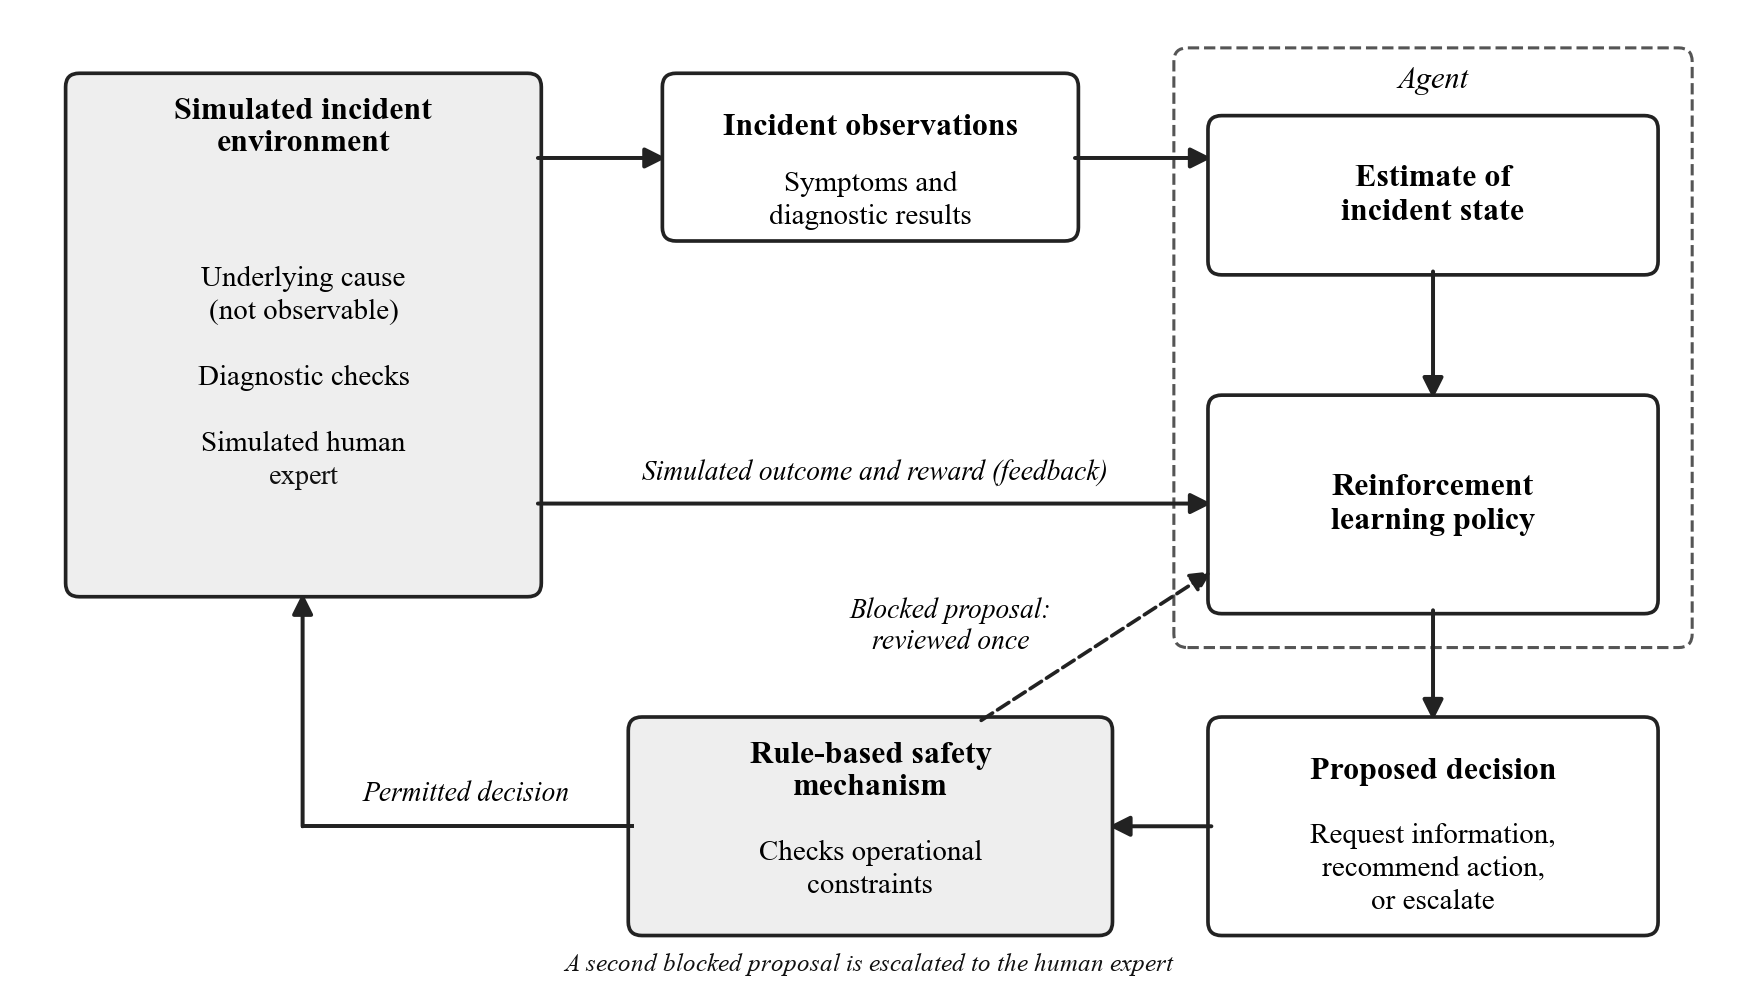
\includegraphics[width=\textwidth]{Figure_1_1_Conceptual_Framework.png}
\caption{Proposed Architecture}
\label{fig:framework}
\end{figure}

\section{The Reinforcement Learning Agents}
\label{sec:agent}

Two learning algorithms are used: a deep Q-network as the primary learner and proximal policy optimisation as a secondary learner, to show whether the findings depend on the choice of algorithm. Both are taken from an established open-source library to limit implementation error~\cite{raffin2021}. Both use action masking: at step $t$ the agent may only choose from the available actions
\begin{equation}
\mathcal{A}_t = \mathcal{A} \setminus \big( \{ a^{\text{chk}}_j : q_{t,j} = 1 \} \cup \mathcal{B}_t \big),
\label{eq:mask}
\end{equation}
which exclude checks already requested and the set $\mathcal{B}_t$ of proposals blocked at this step.

\subsection{Deep Q-Network:}

The deep Q-network (DQN) estimates the action-value function, the expected discounted return of taking action $a$ after observation $o$ and following policy $\pi$ afterwards~\cite{mnih2015}:
\begin{equation}
Q^{\pi}(o, a) = \mathbb{E}_{\pi}\!\left[ \sum_{t' \ge t} \gamma^{t'-t} r_{t'} \;\middle|\; o_t = o,\; a_t = a \right].
\end{equation}
The optimal action values satisfy the Bellman optimality equation, here with the maximum taken only over available actions:
\begin{equation}
Q^{*}(o, a) = \mathbb{E}\!\left[ r_t + \gamma \max_{a' \in \mathcal{A}_{t+1}} Q^{*}(o_{t+1}, a') \;\middle|\; o_t = o,\; a_t = a \right].
\end{equation}

\textbf{Network.} $Q^{*}$ is approximated by a feed-forward neural network with weights $\mathbf{w}$, which takes the encoded observation $\phi(o) \in \mathbb{R}^{n}$ and returns one value for each of the 36 actions. It has two hidden layers of 128 units with rectified linear (ReLU) activations, $\text{ReLU}(v) = \max(0, v)$:
\begin{align}
\mathbf{h}_1 &= \text{ReLU}\big(\mathbf{W}_1 \phi(o) + \mathbf{b}_1\big), & \mathbf{W}_1 &\in \mathbb{R}^{128 \times n}, \\
\mathbf{h}_2 &= \text{ReLU}\big(\mathbf{W}_2 \mathbf{h}_1 + \mathbf{b}_2\big), & \mathbf{W}_2 &\in \mathbb{R}^{128 \times 128}, \\
Q(o, \cdot\,; \mathbf{w}) &= \mathbf{W}_3 \mathbf{h}_2 + \mathbf{b}_3, & \mathbf{W}_3 &\in \mathbb{R}^{|\mathcal{A}| \times 128},
\end{align}
where $\mathbf{w} = \{\mathbf{W}_1, \mathbf{b}_1, \mathbf{W}_2, \mathbf{b}_2, \mathbf{W}_3, \mathbf{b}_3\}$. A tabular method is ruled out because the check states alone admit $4^{20}$ combinations, and the network's output gives a value for every action, so the values the agent assigns to a blocked fix and to escalation can be inspected.

\textbf{Choosing actions.} During training the agent follows an $\epsilon$-greedy policy over the available actions: with probability $1 - \epsilon$ it proposes
\begin{equation}
a_t = \arg\max_{a \in \mathcal{A}_t} Q(o_t, a; \mathbf{w}),
\end{equation}
and with probability $\epsilon$ it proposes an available action chosen uniformly at random. The exploration rate $\epsilon$ decreases during training, and at evaluation $\epsilon = 0$.

\textbf{Learning.} Each transition $(o_t, a_t, r_t, o_{t+1})$ is stored in a replay buffer $\mathcal{E}$, from which mini-batches are sampled. The learning target uses a separate target network with weights $\mathbf{w}^{-}$, copied from $\mathbf{w}$ at fixed intervals, and is masked in the same way as action choice:
\begin{equation}
\tau_t = \begin{cases}
r_t & \text{if } o_{t+1} \text{ is terminal}, \\
r_t + \gamma \max_{a' \in \mathcal{A}_{t+1}} Q(o_{t+1}, a'; \mathbf{w}^{-}) & \text{otherwise}.
\end{cases}
\end{equation}
The weights are updated by gradient descent on the loss
\begin{equation}
\mathcal{L}(\mathbf{w}) = \mathbb{E}_{(o_t, a_t, r_t, o_{t+1}) \sim \mathcal{E}} \Big[ \big( \tau_t - Q(o_t, a_t; \mathbf{w}) \big)^{2} \Big],
\label{eq:dqnloss}
\end{equation}
for which the library uses the Huber form, which is quadratic for small errors and linear for large ones and so limits the effect of outlying targets. The full training loop, with the safety mechanism, is given as Algorithm~\ref{alg:dqn}.

\subsection{Proximal Policy Optimisation:}

Proximal policy optimisation (PPO) learns the policy directly rather than through action values~\cite{schulman2017}. It uses a policy network with weights $\boldsymbol{\vartheta}$ and a value network with weights $\boldsymbol{\psi}$, each with the same two hidden layers of 128 units as the DQN. The policy network outputs a score $f_a(o)$ for each action, and invalid actions are masked by giving them zero probability~\cite{huang2022}:
\begin{equation}
\pi_{\boldsymbol{\vartheta}}(a \mid o_t) = \frac{\exp f_a(o_t)}{\sum_{a' \in \mathcal{A}_t} \exp f_{a'}(o_t)} \quad \text{for } a \in \mathcal{A}_t, \qquad \pi_{\boldsymbol{\vartheta}}(a \mid o_t) = 0 \text{ otherwise}.
\end{equation}
The value network $V_{\boldsymbol{\psi}}(o)$ estimates the expected return from $o$. How much better an action was than expected is measured by the advantage, estimated with generalised advantage estimation~\cite{schulman2016}:
\begin{equation}
\delta_t = r_t + \gamma V_{\boldsymbol{\psi}}(o_{t+1}) - V_{\boldsymbol{\psi}}(o_t), \qquad
\hat{A}_t = \sum_{l=0}^{T-t-1} (\gamma \lambda_{\text{GAE}})^{l}\, \delta_{t+l},
\end{equation}
where $\lambda_{\text{GAE}} \in [0, 1]$ trades bias against variance. PPO limits how far one update can move the policy by clipping the probability ratio between the new and the old policy:
\begin{equation}
\kappa_t(\boldsymbol{\vartheta}) = \frac{\pi_{\boldsymbol{\vartheta}}(a_t \mid o_t)}{\pi_{\boldsymbol{\vartheta}_{\text{old}}}(a_t \mid o_t)}, \qquad
\mathcal{L}^{\text{CLIP}}(\boldsymbol{\vartheta}) = \mathbb{E}_t\Big[ \min\big( \kappa_t \hat{A}_t,\; \text{clip}(\kappa_t, 1 - \epsilon_{\text{clip}}, 1 + \epsilon_{\text{clip}})\, \hat{A}_t \big) \Big].
\end{equation}
The two networks are trained together by maximising
\begin{equation}
\mathcal{L}(\boldsymbol{\vartheta}, \boldsymbol{\psi}) = \mathcal{L}^{\text{CLIP}}(\boldsymbol{\vartheta}) - \nu_1\, \mathbb{E}_t\Big[ \big( V_{\boldsymbol{\psi}}(o_t) - \hat{G}_t \big)^{2} \Big] + \nu_2\, \mathbb{E}_t\Big[ \mathcal{H}\big(\pi_{\boldsymbol{\vartheta}}(\cdot \mid o_t)\big) \Big],
\end{equation}
where $\hat{G}_t = \hat{A}_t + V_{\boldsymbol{\psi}}(o_t)$ is the target return, $\mathcal{H}$ is the entropy of the policy, which encourages exploration, and $\nu_1$ and $\nu_2$ are weighting coefficients.

\subsection{Training:}

Training begins from the library's default hyperparameters, and a small search over the learning rate, the network size and the exploration schedule is carried out on seeds that are not used in the final experiments. The training length is set in pilot runs as the point at which the mean return stops improving. Each agent will be trained with ten random seeds in two regimes: at the base ambiguity level $\ell_0$, and with $\ell$ drawn at random from its planned ranges at the start of each episode. Comparing the two regimes shows whether robustness requires exposure to ambiguity during training. Table~\ref{tab:agentsymbols} summarises the symbols introduced for the agents.

{\small
\begin{longtable}{|P{2.8cm}|P{12.2cm}|}
\caption{Symbols used for the problem, the environment and the agents}
\label{tab:agentsymbols} \\
\hline
\textbf{Symbol} & \textbf{Meaning} \\ \hline
\endfirsthead
\hline
\textbf{Symbol} & \textbf{Meaning} \\ \hline
\endhead
\multicolumn{2}{r}{\emph{Continued on next page}} \\
\endfoot
\endlastfoot
\multicolumn{2}{|l|}{\textit{Problem and environment}} \\ \hline
$\mathcal{C}$, $c_m$, $K$ & Set of causes, the $m$-th cause, number of causes \\ \hline
$c$ & The hidden true cause of the current incident \\ \hline
$\mathcal{D}$, $d_j$, $J$, $k_j$ & Set of diagnostic checks, the $j$-th check, number of checks, cost of check $d_j$ \\ \hline
$\mathcal{X}$, $x$ & Set of incident contexts, the context of the current incident \\ \hline
$\theta_{jm}$ & Probability that check $d_j$ is positive when the cause is $c_m$ \\ \hline
$\sigma_e$, $E$, $\varphi_{em}$ & The $e$-th symptom (1 if present); number of symptoms; probability that symptom $e$ is present when the cause is $c_m$ \\ \hline
$s_t$, $\mathbf{z}$, $\mathbf{q}_t$ & State at step $t$; vector of check results; vector of checks requested by step $t$ \\ \hline
$\mathcal{A}$, $a_t$ & Set of actions; action proposed at step $t$ \\ \hline
$a^{\text{chk}}_j$, $a^{\text{fix}}_m$, $a_{\text{esc}}$ & Request check $d_j$; recommend the fix for cause $c_m$; escalate \\ \hline
$o_t$, $\mathbf{u}_t$, $\boldsymbol{\sigma}$, $\beta_t$ & Observation at step $t$; check states; symptoms; blocked flag \\ \hline
$\phi(o_t)$, $n$ & Encoded observation vector and its length \\ \hline
$r_t$, $r_{\text{correct}}$, $\lambda_{\text{wrong}}$, $\lambda_{\text{esc}}$, $\lambda_{\text{block}}$ & Reward at step $t$; reward for a correct fix; penalty for a wrong fix; cost of an escalation; penalty for a blocked proposal \\ \hline
$\gamma$, $H$, $T$ & Discount factor; step limit; length of an episode \\ \hline
$b_t(c_m)$, $\mathcal{I}_t$ & Belief that the cause is $c_m$ at step $t$; checks whose results have been observed by step $t$ \\ \hline
$\rho_q$, $N_\rho$ & The $q$-th operational rule; number of rules \\ \hline
$\mathcal{A}_{\text{safe}}$ & Actions permitted by all the rules \\ \hline
$a^{(1)}_t$, $a^{(2)}_t$, $a^{\text{exec}}_t$ & First proposal, second proposal and action carried out at step $t$ \\ \hline
$\mathcal{A}_t$, $\mathcal{B}_t$ & Available actions at step $t$; proposals blocked at step $t$ \\ \hline
$\eta(\pi)$ & Expected discounted return of policy $\pi$ \\ \hline
$p_{\text{miss}}$, $p_{\text{noise}}$, $\omega$ & Probabilities that a check is missing or reversed; overlap between causes in a category \\ \hline
$\tilde{\theta}_{jm}$, $\theta'_{jm}$, $\varphi'_{em}$, $g(m)$ & Check likelihood after noise; check and symptom likelihoods after overlap; category of cause $c_m$ \\ \hline
$y$ & Reference label: 1 if the incident should be escalated \\ \hline
\multicolumn{2}{|l|}{\textit{Deep Q-network}} \\ \hline
$Q^{\pi}(o,a)$, $Q^{*}$ & Action value under policy $\pi$; optimal action value \\ \hline
$\mathbf{w}$, $\mathbf{w}^{-}$ & Weights of the Q-network and of the target network \\ \hline
$\mathbf{W}_\cdot$, $\mathbf{b}_\cdot$, $\mathbf{h}_\cdot$ & Weight matrices, bias vectors and hidden-layer outputs \\ \hline
$\epsilon$ & Exploration rate of the $\epsilon$-greedy policy \\ \hline
$\mathcal{E}$, $\tau_t$, $\mathcal{L}$ & Replay buffer; learning target; loss \\ \hline
\multicolumn{2}{|l|}{\textit{Proximal policy optimisation}} \\ \hline
$\boldsymbol{\vartheta}$, $\boldsymbol{\psi}$ & Weights of the policy network and of the value network \\ \hline
$f_a(o)$, $\pi_{\boldsymbol{\vartheta}}$, $V_{\boldsymbol{\psi}}$ & Score of action $a$; policy; value estimate \\ \hline
$\delta_t$, $\hat{A}_t$, $\lambda_{\text{GAE}}$ & Temporal-difference error; estimated advantage; advantage-estimation parameter \\ \hline
$\kappa_t$, $\epsilon_{\text{clip}}$ & Probability ratio between new and old policy; clipping range \\ \hline
$\hat{G}_t$, $\mathcal{H}$, $\nu_1$, $\nu_2$ & Target return; policy entropy; loss weights \\ \hline
\end{longtable}
}

\section{Baseline Decision Policies}
\label{sec:baselines}

The agent will be compared with six baseline policies that run in the same environment on the same evaluation incidents, each standing for an approach from Chapter~2 (Table~\ref{tab:baselines}).

\begin{table}[H]
\centering
\caption{Baseline decision policies}
\label{tab:baselines}
\small
\begin{tabular}{|p{3.4cm}|p{7.4cm}|p{4.2cm}|}
\hline
\textbf{Policy} & \textbf{Behaviour} & \textbf{Approach represented} \\ \hline
Initial-symptom & Recommends the fix for the cause that the prior and the symptoms make most likely (Equation~\eqref{eq:belief} at $t = 0$), without checks & Triage as one prediction \\ \hline
Scripted checklist & Requests a fixed sequence of checks for the category, elicited from Directorate practice, then recommends & Runbook practice \\ \hline
Always-escalate & Escalates every incident & The limit of deferral \\ \hline
Confidence threshold & Tracks the belief $b_t$ of Equation~\eqref{eq:belief}, requests the most informative check until one cause passes a threshold, else escalates & Uncertainty-driven investigation (knows the model) \\ \hline
Unconstrained agent & The same DQN without the safety mechanism & Standard shielding comparison \\ \hline
Penalty-only agent & The same DQN without the mechanism, with a reward penalty per rule violation & Constraint by reward penalty \\ \hline
\end{tabular}
\end{table}

The confidence-threshold policy is given as Algorithm~\ref{alg:threshold}. Two ablations of the agent, one that cannot request checks and one that cannot escalate, will show what each option contributes.

\section{Evaluation Strategy}
\label{sec:evaluation}

The framework will be evaluated across four groups of measures: decision quality, investigation efficiency, escalation behaviour and constraint compliance. At each level of ambiguity, $S = 10$ evaluation sets of $N = 1{,}000$ incidents each are generated from seeds never used in training, and every policy is run on the same sets. Set $s$ is paired with training seed $s$ of each learning agent; a baseline that does not learn is run on all $S$ sets, so that every policy has $S$ values of each measure. With $N = 1{,}000$, the standard error of a rate measured on one set is at most $\sqrt{0.25/1000} \approx 0.016$, small enough to resolve the differences of 0.05 used in the decision criteria (Section~\ref{sec:criteria}). Each episode $i$ ends in one of three outcomes $o_i$: a correct recommendation (c), a wrong recommendation (w) or an escalation (e). Let $N_{\text{c}}$, $N_{\text{w}}$ and $N_{\text{e}}$ be the numbers of episodes with each outcome, so that
\begin{equation}
N = N_{\text{c}} + N_{\text{w}} + N_{\text{e}}.
\end{equation}
Escalations include those chosen by the agent, those forced by the safety mechanism and those caused by the step limit. Table~\ref{tab:notation} defines the symbols used in the rest of this section.

{\small
\begin{longtable}{|P{2.6cm}|P{12.4cm}|}
\caption{Symbols used in the evaluation measures}
\label{tab:notation} \\
\hline
\textbf{Symbol} & \textbf{Meaning} \\ \hline
\endfirsthead
\hline
\textbf{Symbol} & \textbf{Meaning} \\ \hline
\endhead
\multicolumn{2}{r}{\emph{Continued on next page}} \\
\endfoot
\endlastfoot
\multicolumn{2}{|l|}{\textit{Episodes and outcomes}} \\ \hline
$N$ & Number of incidents in one evaluation set ($N = 1{,}000$); each episode is the triage of one incident \\ \hline
$i$ & Index of an evaluation episode, $i = 1, \dots, N$ \\ \hline
$o_i$ & Outcome of episode $i$: c (correct recommendation), w (wrong recommendation) or e (escalation) \\ \hline
$N_{\text{c}}, N_{\text{w}}, N_{\text{e}}$ & Numbers of episodes ending in a correct recommendation, a wrong recommendation and an escalation \\ \hline
$T_i$ & Number of steps taken in episode $i$ \\ \hline
$r_{i,t}$ & Reward received at step $t$ of episode $i$ \\ \hline
$\pi$ & A decision policy: the proposed agent or one of the baselines \\ \hline
\multicolumn{2}{|l|}{\textit{Investigation}} \\ \hline
$K_i$ & Set of diagnostic checks requested in episode $i$; $|K_i|$ is their number \\ \hline
$k_j$ & Cost of diagnostic check $j$ \\ \hline
\multicolumn{2}{|l|}{\textit{Escalation}} \\ \hline
$y_i$ & Reference label of episode $i$: 1 if the incident should be escalated, 0 otherwise \\ \hline
$\hat{y}_i$ & Agent's choice in episode $i$: 1 if it chose to escalate, 0 otherwise \\ \hline
TP, FP, FN, TN & True positives, false positives, false negatives and true negatives: the four cells of the confusion matrix of $\hat{y}_i$ against $y_i$ \\ \hline
\multicolumn{2}{|l|}{\textit{Constraint compliance}} \\ \hline
$M$ & Total number of actions proposed by the agent over the evaluation episodes \\ \hline
$M_{\text{b}}$ & Number of proposed actions blocked by the safety mechanism \\ \hline
$N_{\text{f}}$ & Number of episodes ending in a forced escalation after a second blocked proposal \\ \hline
$N_{\text{v}}$ & Number of episodes in which a prohibited action took effect \\ \hline
$v_i$ & 1 if a prohibited action took effect in episode $i$, 0 otherwise \\ \hline
$\mathbf{1}[\cdot]$ & Indicator function: 1 when the condition in brackets holds, 0 otherwise \\ \hline
\multicolumn{2}{|l|}{\textit{Robustness and reporting}} \\ \hline
$\ell$ & Level of ambiguity, set by $p_{\text{miss}}$, $p_{\text{noise}}$ and $\omega$ (Section~\ref{sec:environment}) \\ \hline
$\ell_0$ & Base level of ambiguity, at which the agent is trained in the first regime \\ \hline
$S$ & Number of training seeds per learning agent, and of evaluation sets per ambiguity level ($S = 10$) \\ \hline
$s$ & Index of a seed, $s = 1, \dots, S$ \\ \hline
$X$, $X_s$, $\bar{X}$ & Any measure; its value on seed $s$; its mean over seeds \\ \hline
$B$ & Number of bootstrap resamples used for the confidence interval ($B = 10{,}000$) \\ \hline
\multicolumn{2}{|l|}{\textit{Measures}} \\ \hline
Acc & Resolution accuracy \\ \hline
Cov & Coverage: share of incidents on which the agent makes a recommendation \\ \hline
SelAcc & Selective accuracy: accuracy of the recommendations made \\ \hline
WR & Wrong-recommendation rate \\ \hline
$\bar{G}$ & Mean episodic return \\ \hline
$\bar{n}$, $\bar{C}$ & Mean number of checks and mean investigation cost per episode \\ \hline
ER & Escalation rate \\ \hline
$P$, $R$, $F_1$ & Escalation precision, recall and F1 score \\ \hline
MCC & Matthews correlation coefficient of escalations \\ \hline
PVR & Proposed-violation rate \\ \hline
FER & Forced-escalation rate \\ \hline
EVR & Executed-violation rate \\ \hline
CSR & Compliant success rate \\ \hline
$\Delta\text{Acc}(\ell)$ & Change in resolution accuracy at level $\ell$ relative to $\ell_0$ \\ \hline
$\mathbf{m}(\ell)$ & Decision mix at level $\ell$: coverage, escalation rate and mean number of checks \\ \hline
\end{longtable}
}

\subsection{Decision Quality:}

Decision quality describes how often the final decision is right. Resolution accuracy is the share of all incidents that the agent resolves itself, the usual accuracy of the triage literature~\cite{remil2024}:
\begin{equation}
\text{Acc} = \frac{N_{\text{c}}}{N}.
\end{equation}
Because an agent can avoid errors by escalating, accuracy is read together with coverage and selective accuracy, the standard pair of selective prediction~\cite{geifman2019}:
\begin{equation}
\text{Cov} = \frac{N_{\text{c}} + N_{\text{w}}}{N}, \qquad
\text{SelAcc} = \frac{N_{\text{c}}}{N_{\text{c}} + N_{\text{w}}}.
\end{equation}
The wrong-recommendation rate isolates the most costly error in triage:
\begin{equation}
\text{WR} = \frac{N_{\text{w}}}{N}.
\end{equation}
The mean episodic return is the quantity the agent is trained to maximise~\cite{sutton2018}:
\begin{equation}
\bar{G} = \frac{1}{N}\sum_{i=1}^{N}\sum_{t=0}^{T_i-1} r_{i,t},
\end{equation}
where $T_i$ is the number of steps in episode $i$ and $r_{i,t}$ is the reward at step $t$. Because $\bar{G}$ depends on the reward values chosen, it is never reported alone.

\subsection{Investigation Efficiency:}

Investigation efficiency describes what the agent spends on evidence before it decides. Let $K_i$ be the set of checks requested in episode $i$ and $k_j$ the cost of check $j$. The mean number of checks and the mean investigation cost are
\begin{equation}
\bar{n} = \frac{1}{N}\sum_{i=1}^{N} |K_i|, \qquad
\bar{C} = \frac{1}{N}\sum_{i=1}^{N}\sum_{j \in K_i} k_j.
\end{equation}
The cost stands in for time, which a simulation without a clock cannot measure directly. Following the evaluation of costly feature acquisition~\cite{janisch2019}, each policy $\pi$ is also plotted as a point $(\bar{C}_\pi, \text{Acc}_\pi)$ on an accuracy--cost curve, which shows whether additional investigation buys additional accuracy and allows policies to be compared at equal cost.

\subsection{Escalation Behaviour:}

Escalation behaviour describes how much the agent hands to the human expert and whether it hands over the right cases. The escalation rate is the load placed on human experts~\cite{turan2026}:
\begin{equation}
\text{ER} = \frac{N_{\text{e}}}{N}.
\end{equation}
The remaining measures compare the agent's own choices with the reference labels. For each episode, let $y_i = 1$ if the incident is labelled as one that should be escalated and $y_i = 0$ otherwise, and let $\hat{y}_i = 1$ if the agent chose to escalate and $\hat{y}_i = 0$ otherwise. Forced escalations and step-limit escalations are excluded, because the agent did not choose them; they are reported under constraint compliance. Over the remaining episodes,
\begin{equation}
\text{TP} = \sum_i \hat{y}_i\, y_i, \quad
\text{FP} = \sum_i \hat{y}_i (1-y_i), \quad
\text{FN} = \sum_i (1-\hat{y}_i)\, y_i, \quad
\text{TN} = \sum_i (1-\hat{y}_i)(1-y_i).
\end{equation}
Escalation precision is the share of the agent's escalations that should have been escalated; low precision means that human experts receive incidents the agent could have resolved. Escalation recall is the share of incidents that should have been escalated that the agent did escalate; low recall means the agent kept incidents it should have handed over. The F1 score is their harmonic mean:
\begin{equation}
P = \frac{\text{TP}}{\text{TP}+\text{FP}}, \qquad
R = \frac{\text{TP}}{\text{TP}+\text{FN}}, \qquad
F_1 = \frac{2PR}{P+R}.
\end{equation}
Because precision, recall and F1 can all look acceptable when one class is rare, the Matthews correlation coefficient, which uses all four cells of the confusion matrix and exposed degenerate triage policies that F1 concealed~\cite{okafor2026}, is also reported:
\begin{equation}
\text{MCC} = \frac{\text{TP}\cdot\text{TN} - \text{FP}\cdot\text{FN}}
{\sqrt{(\text{TP}+\text{FP})(\text{TP}+\text{FN})(\text{TN}+\text{FP})(\text{TN}+\text{FN})}}.
\end{equation}
MCC ranges from $-1$ to $+1$, where $0$ means the agent's escalations are no better than chance.

\subsection{Constraint Compliance:}

Constraint compliance describes the agent's relationship to the rules. Let $M$ be the total number of actions the agent proposes over the evaluation episodes and $M_{\text{b}}$ the number blocked by the safety mechanism. The proposed-violation rate shows whether the agent has learned to act within the rules or relies on being stopped:
\begin{equation}
\text{PVR} = \frac{M_{\text{b}}}{M}.
\end{equation}
Let $N_{\text{f}}$ be the number of episodes that end in a forced escalation after a second blocked proposal, and $N_{\text{v}}$ the number in which a prohibited action takes effect. The forced-escalation rate and the executed-violation rate are
\begin{equation}
\text{FER} = \frac{N_{\text{f}}}{N}, \qquad
\text{EVR} = \frac{N_{\text{v}}}{N}.
\end{equation}
The executed-violation rate is zero by construction when the mechanism is active, and it is the central measure for the unconstrained and penalty-only agents, as in the shielding literature~\cite{alshiekh2018}. Let $v_i = 1$ if a prohibited action took effect in episode $i$. The compliant success rate, which follows the measure of task completion under policy used for agent benchmarks~\cite{levy2026}, is
\begin{equation}
\text{CSR} = \frac{1}{N}\sum_{i=1}^{N} \mathbf{1}\left[o_i = \text{c} \;\wedge\; v_i = 0\right],
\end{equation}
where $\mathbf{1}[\cdot]$ equals 1 when its condition holds and 0 otherwise. For agents without the mechanism, the gap between Acc and CSR shows how much of their accuracy was obtained by breaking rules.

\subsection{Robustness:}

Robustness is not a separate metric: every measure above is computed at each ambiguity level $\ell$ and reported as a function of it. Degradation is the change relative to the base level $\ell_0$, for example
\begin{equation}
\Delta\text{Acc}(\ell) = \text{Acc}(\ell) - \text{Acc}(\ell_0),
\end{equation}
and likewise for the wrong-recommendation rate. The decision mix at each level,
\begin{equation}
\mathbf{m}(\ell) = \big(\text{Cov}(\ell),\; \text{ER}(\ell),\; \bar{n}(\ell)\big),
\end{equation}
shows whether the agent responds to ambiguity by investigating more, by escalating more, or by continuing to recommend on weaker evidence, which is the behaviour tested by hypotheses H3a to H3c.

\subsection{Reporting:}

Each learning agent is trained with $S = 10$ random seeds, and each seed is evaluated on its paired evaluation set. For any measure $X$, the reported value is the mean over the $S$ values,
\begin{equation}
\bar{X} = \frac{1}{S}\sum_{s=1}^{S} X_s,
\end{equation}
with a 95\% percentile bootstrap confidence interval obtained by resampling the $S$ values with replacement $B = 10{,}000$ times and taking the 2.5th and 97.5th percentiles of the resampled means~\cite{agarwal2021}.

\subsection{Decision Criteria:}
\label{sec:criteria}

The hypotheses are judged by the following criteria, fixed before any experiment is run. A policy is said to score \emph{higher} than another on a rate when its mean exceeds the other's by at least 0.05 and the two 95\% bootstrap confidence intervals do not overlap; \emph{lower} is defined in the same way. For the mean number of checks, the minimum difference is 0.5 checks. Any other outcome counts as no difference.
\begin{itemize}
\item \textbf{H1} is supported if, at $\ell_0$, the agent's resolution accuracy is higher than that of each of the initial-symptom, scripted-checklist and always-escalate policies, and its mean investigation cost is not higher than that of the scripted checklist. Otherwise it is not supported.
\item \textbf{H2} is supported if, at $\ell_0$, the agent's compliant success rate is higher than that of both the unconstrained agent and the penalty-only agent. The executed-violation rate of the agent with the mechanism is checked separately as a verification of the implementation: it must be zero on every evaluation incident, and any other value is treated as a defect to be corrected before results are reported.
\item \textbf{H3a to H3c} are judged one factor at a time, by comparing the agent at $\ell_0$ with the agent at the highest planned value of the factor concerned, the other two factors held at their base values. H3a is supported if, as $p_{\text{miss}}$ rises, the escalation rate is higher and the mean number of checks is not higher. H3b is supported if, as $p_{\text{noise}}$ rises, the mean number of checks is higher and coverage is lower. H3c is supported if, as $\omega$ rises, the mean number of checks and the escalation rate are both higher.
\end{itemize}
Each hypothesis is reported as supported or not supported, whichever the results show.

\subsection{Experiments:}

Four experiments use these measures. Experiment~1 compares the agent with the six baselines at the base level of ambiguity, and is repeated with the PPO agent to check that the findings do not depend on the learning algorithm. Experiment~2 compares the agent with the unconstrained and penalty-only agents and tracks the proposed-violation rate over training. Experiment~3 compares it with its two ablations. Experiment~4 evaluates every policy across ambiguity levels, for both training regimes. Its sweep is one factor at a time from $\ell_0$: each control takes its three non-base planned values while the other two stay at their base values, giving nine levels, which with $\ell_0$ make ten. Two combined levels are added, with all three controls at their second-highest and at their highest planned values, giving twelve ambiguity settings in all. A sensitivity analysis repeats Experiment~1 with the escalation cost set to $\lambda_{\text{esc}} \in \{1, 3, 6, 9\}$, all below $\lambda_{\text{wrong}}$. All measures are computed on the evaluation sets described at the start of this section, following Algorithm~\ref{alg:evaluation}.

\section{Limitations}
\label{sec:limitations}

The design has limitations that bound what its results can show.
\begin{itemize}[nosep]
\item \textbf{Simulation and reality.} The agent is trained and evaluated only in a simulator built from staff ratings, so the results show how it behaves in that model, not how it would perform at the Directorate.
\item \textbf{An expert who always succeeds.} The simulated human expert resolves every escalated incident, so escalation is never itself a source of error, and its only cost is $\lambda_{\text{esc}}$.
\item \textbf{A low cost of escalation.} With $\lambda_{\text{esc}} = 3$ against $\lambda_{\text{wrong}} = 10$, escalation is cheap relative to a wrong fix, which may understate its burden on experts and encourage escalation; the sensitivity analysis over $\lambda_{\text{esc}} \in \{1, 3, 6, 9\}$ shows how far the conclusions depend on this value.
\item \textbf{Conditional independence.} Symptoms and check results are assumed to be independent given the cause. In practice, checks that read the same logs may be correlated, which would make evidence less informative than the simulator assumes.
\item \textbf{Researcher-chosen rewards.} The reward values are set by the researcher and tuned in pilot runs, not measured at the Directorate, and the agent's behaviour depends on them.
\item \textbf{One institution.} The scenario model comes from a single IT directorate, so its causes, checks, rules and ratings may not represent other organisations.
\end{itemize}
